\RequirePackage[T1]{fontenc}
\documentclass[journal]{IEEEtran}
\usepackage{amsmath,amssymb,booktabs,cite,xurl,graphicx}
\usepackage[hidelinks]{hyperref}
\interdisplaylinepenalty=2500
\begin{document}
\title{Segment Running Time Estimation with Known Total Duration and Information Sharing across Repeated Segments}
\author{}
\maketitle
\begin{abstract}
Bus operation analysis needs to locate intervals with long running times, although sparse observations often cover only a whole trip and a few local positions. A known running-time total does not uniquely determine interval times, and repeated intervals vary across trips. Ours combines estimates shared across repeated intervals with bounded trip-specific redistribution, followed by proportional scaling to the known total. Development-set experiments on public Astana bus data compare three local-label budgets. In the validation-selected main comparison, Ours has lower point-estimate mean absolute error than same-input direct prediction at 1\% and 5\% (by 0.579 and 0.075 seconds) but higher error at 10\%; paired runs favor Ours in eight, six, and zero of nine runs, respectively. Identity means remain stronger at 1\%. A validation-selected 0.5-weight Ours+Direct ensemble has lower development-set MAE than direct prediction at all three budgets, but it is a separate predictor and does not outperform identity means at 1\%. Equal label counts also yield different errors when interval coverage changes. The final chronological split remains unopened, so these results are limited to development comparisons.
\end{abstract}
\begin{IEEEkeywords}
Segment running time estimation, known total duration, segment information sharing, sparse supervision, bus operations.
\end{IEEEkeywords}
\section{Introduction}
Bus operators need to know where time is spent along a route. A trip total supports comparisons of operating efficiency, but cannot show whether a particular delay occurred near the beginning or the end. Interval running times support bottleneck screening and comparisons across departure periods. Obtaining complete local records, however, requires continuous position observations and reliable stop matching. Sampling intervals and missing records leave some parts of a trip unobserved. Estimating segment times from a known total and limited local observations is therefore a practical need in travel-time inference\cite{hellinga2008,hofleitner2011,yin2015entryexit}.

We study segment running times for completed trips. A segment denotes a directed inter-stop interval, and the known total is the sum of interval running times, excluding dwell. This differs from the elapsed time between endpoint timestamps, which can include dwell and other non-running time. Using such a measurement requires separating those components and aligning the interval boundaries. Our experiments sum public running-time labels to evaluate interval estimation under an exact known total.

Consider a trip through three consecutive intervals with a total running time of ten minutes. Both $(2,3,5)$ and $(5,3,2)$ minutes remain feasible. A training label of three minutes at the middle position still cannot distinguish these allocations; current-trip local labels are unavailable at inference. The two allocations identify different intervals as the most time-consuming and can lead to different operating decisions. Records of the same intervals in other trips help distinguish the alternatives. Yet changes in departure period or route context can make a historical average unrepresentative of the current trip. This example calls for both information sharing across repeated intervals and an estimate of how the current trip departs from that shared pattern.

Earlier methods use free-flow information, local time distributions, or statistical traffic-flow models to inform total-time decomposition\cite{hellinga2008,hofleitner2011}. When paths are incomplete, link inference must also recover the traveled path\cite{yin2015entryexit,sun2022prltte}. We focus on known ordered paths with recurring interval identities and a subset of observed singleton labels. Path recovery is unnecessary in this setting. The remaining question is how to combine information shared across trips with current-trip variation while making interval outputs consistent with the known total.

A segment mean shares repeated observations but treats context-varying durations as fixed. Our direct sequence baseline also shares interval embeddings and uses current-trip context, but outputs positive scores without a separate redistribution branch. We separate these roles: a shared branch estimates contextual base times, and a sequence branch proposes bounded redistribution before proportional rescaling to the known total. The contribution is this allocation parameterization and its analysis under sparse labels; an accuracy advantage over direct prediction is an empirical question.

The experiments further delimit the role of this design. Segment means remain competitive when local labels are scarce. At larger budgets, our method improves on segment means but shows no consistent advantage over same-input direct prediction. Disabling trip correction increases the error of the same model, indicating that the correction helps the base estimate; this comparison does not establish that the complete method is better than direct prediction. The same number of labels also produces substantially different errors when it covers fewer interval identities. In a control that preserves the identity set and the count for each identity, randomizing label positions does not recover the accuracy obtained with broader coverage. A known total rules out allocations that violate the sum, but cannot by itself determine which local allocation is correct; useful local estimates also depend on how well repeated intervals are represented in the supervision.

\section{Related Work}
\subsection{Decomposition of Observed Travel Times}
Sparse probe observations can span several road links, requiring the elapsed time between observations to be allocated along an identified path. Hellinga et al.\ separate free-flow, congestion, and stopping time using link geometry and free-flow speeds\cite{hellinga2008}. Their congestion likelihood uses the preceding polling interval, while the stopping likelihood reflects the vehicle's position relative to the downstream end of a link. The resulting allocation integrates over possible congestion levels. Hofleitner and Bayen instead derive link-time distributions from a statistical model of arterial queues and driving behavior\cite{hofleitner2011}. These distributions are mixtures of log-concave components. The mixture allocation problem is nonconvex, but fixed delay patterns yield convex subproblems that support enumeration and EM-based algorithms. Both studies constrain allocated times to the observed duration.

Network-level inference also uses observations shared across trips. Yin et al.\ infer link-time distributions from entry and exit records, using Gaussian likelihoods, mixture estimation when paths are unknown, and trip splitting for more general distributions\cite{yin2015entryexit}. PR-LTTE alternates path recovery from trip distance and duration with nonnegative least-squares link-time estimation\cite{sun2022prltte}. These methods estimate shared road-link quantities and may recover missing paths. The present study assumes an ordered sequence of directed bus inter-stop intervals, each of which may span several road links. Its shared estimates vary with observed context, and its redistribution varies with the trip. The NNLS-Ridge reference examines fixed interval-identity coefficients under this known-sequence setting.

\subsection{Learned Travel-Time Representations}
DeepTTE combines geographic convolution and recurrent layers with joint whole-path and local-path supervision\cite{wang2018deeptte}. Its local targets are timestamp differences over GPS windows, which can overlap; the whole-path prediction is produced by a separate attention-based head. DutyTTE addresses uncertainty when the route is not supplied, combining predicted-path alignment with contextual segment uncertainty\cite{mao2025dutytte}. These designs show how local observations and route representations can support prediction of an unknown trip duration.

ProbETA provides a closer connection to sharing information across repeated links\cite{xu2025probeta}. Xu et al.\ model link travel time as a shared mean plus day-specific and trip-specific Gaussian effects. Learned low-rank covariance representations express dependencies both across trips and within a trip. Training uses joint likelihoods of trip durations and timestamp-derived sub-trip durations; inference conditions the queried trip's distribution on nearby completed trips. This is a probabilistic use of shared link evidence. In our setting, the queried total is already supplied, and limited singleton labels supervise the allocation. The trip correction is bounded relative to a shared contextual base and sums to zero within that trip, rather than parameterizing a covariance distribution.

\subsection{Aggregate Supervision and Consistent Outputs}
Learning from aggregate observations formalizes the estimation of individual labels from group-level supervision. Zhang et al.\ derive a likelihood for the observed aggregate and study regression from means or sums under conditional independence assumptions\cite{zhang2020aggregate}. Their aggregate error trains the individual predictor. Here, proportional rescaling enforces the supplied total for every output, so a loss on that final sum provides no learning signal. Training and model selection therefore use the visible singleton labels in the training and validation sets, respectively.

Forecast reconciliation offers another way to enforce additive consistency. MinT combines forecasts at different aggregation levels using their error covariance to obtain coherent forecasts\cite{wickramasuriya2019mint}. The present total is an observed input, while the unknown interval shares are learned and then scaled to it. We accordingly compare the shared-base redistribution model with direct interval prediction under the same inputs, label budgets, and final scaling. This comparison examines how the within-trip allocation is learned once consistency is imposed.

\section{Methodology}
\subsection{Task Definition}
Training receives directed inter-stop sequences, contextual features, and trip running-time totals, with supervision from visible singleton interval labels. Inference uses the same input types to estimate the current trip's interval times. An interval connects adjacent stops and may span several road edges. Repeated intervals share parameters to use observations from other trips while allowing their durations to differ.

Trip $q$ contains $L_q$ ordered intervals. Interval $i$ has identity $s_{qi}$, features $x_{qi}$, and running time $t_{qi}\geq0$; the known total is $T_q>0$. Writing the ordered features and identities as $X_q$, the output satisfies
\begin{equation}
\hat{\boldsymbol t}_q=f_\theta(X_q,T_q),\qquad
\hat{\boldsymbol t}_q\geq0,\quad
\boldsymbol1^\top\hat{\boldsymbol t}_q=T_q.
\label{eq:task}
\end{equation}
The total and interval targets use the same time definition and observation boundaries. Local truth from the current trip is not an inference input.

Only positions in $V$ have training labels. With $m<L_q-1$ distinct labeled positions, the local observations and total leave $L_q-m-1$ free directions near a strictly positive feasible allocation. Moving a small amount between two unobserved intervals preserves every observation. This explains the ambiguity between the first and last intervals in the introduction and motivates learning allocation patterns from repeated intervals and context.

\subsection{Overall Design}
Figure~\ref{fig:framework} shows three steps: estimate base times from interval identities and context, adjust their relative allocation using the ordered trip, and normalize the predicted profile to the known total. Both branches receive local supervision through the final outputs. The total is not an encoder feature; information from repeated intervals is accumulated in shared training parameters, without requiring historical target records at inference.
\begin{figure*}[t]
\centering
\rule{0pt}{1.5in}
\caption{Overview of Ours. The shared branch estimates positive base times, and the sequence branch predicts a bounded zero-sum correction. The known trip total is imposed by proportional rescaling.}\label{fig:framework}
\end{figure*}
\subsection{Shared and Sequence Representations}
We construct two representations for each valid component. A shared representation $h^B_{qi}$ combines a common feature mapping with an identity embedding. Its parameters are reused across occurrences of the same identity. A sequence representation $h^R_{qi}$ combines local features, identity and position embeddings, a directed-neighbor transition, and a Transformer encoder. A projected mean of the valid sequence representations is added back to the tokens before layer normalization. Padding is masked throughout.

The base and correction scores are produced by scalar multilayer heads. Let $I_q$ denote valid positions. Suppressing the sequence index,
\begin{align}
 b_i&=\exp\bigl(\operatorname{clip}(g_B(h^B_i),-8,12)\bigr),\\
 u_i&=g_R(h^R_i),\qquad
 z_i=u_i-\frac{1}{|I_q|}\sum_{j\in I_q}u_j,\qquad i\in I_q.
\label{eq:heads}
\end{align}
Clipping protects exponentiation against overflow, and $z_i$ is centered over valid positions. The next step centers local adjustments in proportion to the base to make their sum zero. Because the shared features include calendar context, $b_i$ varies with conditions rather than being a fixed historical mean.

\subsection{Bounded Redistribution}
Let $B=\sum_jb_j$ and $p_i=b_i/B$. With a fixed $0<\rho<1/2$, define
\begin{align}
 a_i&=\rho b_i\tanh(z_i),\\
 \delta_i&=a_i-p_i\sum_j a_j,\qquad r_i=b_i+\delta_i.
\label{eq:redistribution}
\end{align}
The first term proposes a context-dependent local change. The second removes its aggregate component in proportion to the base. Since $\sum_i p_i=1$, the correction satisfies $\sum_i\delta_i=0$ and therefore $\sum_ir_i=B$. Furthermore,
\begin{equation}
 |\delta_i|\leq\rho b_i+p_i\rho B=2\rho b_i,
\end{equation}
which gives
\begin{equation}
 (1-2\rho)b_i\leq r_i\leq(1+2\rho)b_i.
\label{eq:positive}
\end{equation}
Thus every valid corrected component remains strictly positive. The main comparison selects $\rho$ separately for each label budget using visible validation labels; fixed-$\rho=0.45$ controls are reported separately. Setting the correction scores to zero removes this redistribution and leaves the base unchanged.

The amplitude bound keeps trip adjustments related to the base and guarantees positive values. It may also limit correction when the base is severely biased. Zero-sum centering removes the trip branch's aggregate increase or decrease so that it handles redistribution between intervals. Final rescaling guarantees total consistency for any positive vector; centering therefore constrains the correction branch rather than providing a necessary conservation step. Experiments compare amplitudes and centering forms to examine their effect on error.

\subsection{Adjustment to the Known Total}
The base estimates need not sum to the known duration. Proportional rescaling imposes Eq.~\eqref{eq:task},
\begin{equation}
 \hat t_i=T\frac{r_i}{\sum_jr_j}=T\frac{r_i}{B}.
\label{eq:rescaling}
\end{equation}
Equivalently,
\begin{equation}
 \hat t_i=T p_i\left[1+\rho\left(\tanh z_i-\sum_jp_j\tanh z_j\right)\right].
\label{eq:shape}
\end{equation}
Equation~\eqref{eq:shape} shows that the base and centered correction determine within-trip proportions, while $T$ determines their scale. Valid predictions remain nonnegative and padding is zero. Floating-point summation residuals are added to the largest valid component. Changing $T$ with $X$ fixed rescales all predictions proportionally. Ours and direct prediction use the same final adjustment, making local allocation the focus of their comparison.

\subsection{Learning from Visible Local Targets}
For visible training positions $V_{\mathcal B}$ in a batch $\mathcal B$, we minimize
\begin{equation}
 \mathcal L_{\mathcal B}=\frac{1}{|V_{\mathcal B}|}
 \sum_{(q,i)\in V_{\mathcal B}}h_\beta(\hat t_{qi}-t_{qi}),
\label{eq:loss}
\end{equation}
where
\begin{equation}
 h_\beta(e)=
 \begin{cases}e^2/(2\beta),&|e|<\beta,\\ |e|-\beta/2,&\text{otherwise}.
 \end{cases}
\end{equation}
We use $\beta=5$ seconds. Rescaling couples interval predictions through their common denominator, allowing visible errors to propagate into both branches. Hidden labels do not contribute to the objective. Total error after rescaling is identically zero and cannot train the allocation alone; the primary experiment therefore uses local Huber supervision, with uniform allocation as a label-free reference. Redistribution and rescaling require $O(L)$ work, while self-attention requires $O(L^2d)$ for width $d$.

\subsection{Optional Objectives with Complete Labels}
The primary experiment uses only Eq.~\eqref{eq:loss}. The reported Singapore auxiliary runs disable the history sidecar; with complete local labels, they add duration weights and a prefix objective. With $M_{qk}=1$ at valid positions,
\begin{equation}
\mathcal L_P=\frac{\sum_{q,k}M_{qk}\left|\sum_{i\leq k}(\hat t_{qi}-t_{qi})\right|/\max(T_q,1)}{\sum_{q,k}M_{qk}}.
\label{eq:prefix}
\end{equation}
Cumulative errors and the denominator count valid intervals only, making the loss invariant to additional right padding. The auxiliary objective is $\mathcal L_W+\lambda_P\mathcal L_P$, where $\mathcal L_W$ normalizes weighted local Huber errors by the sum of valid duration weights. We specify these weights in the experiments and report the additional-history log-time objective separately in the supplement.

\section{Experiments}
The main comparisons use Astana data with the same local loss and training settings. A Singapore auxiliary experiment evaluates the prefix objective with complete local labels.

\subsection{Data and Time Definitions}
Astana\cite{astana2025} was released on Zenodo on June 29, 2025 under CC BY 4.0, with data collected on three bus routes during July--September 2024. The interval records used here span July 29--September 21, 2024 and contain 785,976 records from 19,769 trips. Preprocessing requires a continuous directed stop chain, running times of 5--1,800 seconds, and dwell times of 0--900 seconds. Trips violating these conditions are removed in full. The resulting sample contains 10,910 trips, 439,659 intervals, and 586 directed interval identities. The longest valid trip has 55 intervals, which sets the padding length; longer trips are not truncated.

Interval identities combine direction and endpoint stop identifiers. Targets use the recorded running-time field, and their sum supplies the input total, excluding dwell. Trips are ordered chronologically and split 60\%/20\%/20\%. From the first 60\%, 5,891 trips are used for fitting and 655 for checkpoint selection; the middle 20\% (2,182 trips) is the development evaluation set. The final 20\% is excluded from the reported results (Table~\ref{tab:partitions}).
\begin{table}[t]
\centering\footnotesize
\caption{Astana partitions and valid-label populations.}\label{tab:partitions}
\begin{tabular}{lrr}\toprule
Role & Trips & Intervals\\\midrule
Model fitting & 5,891 & 237,203\\
Checkpoint selection & 655 & 26,561\\
Development evaluation & 2,182 & 87,715\\
\bottomrule\end{tabular}
\end{table}

Models use 31 geometry, route, stop, and departure-calendar features. Normalization is estimated from fitting features only. Inputs exclude target-derived statistics, actual interval entry times, label-quality fields, and additional historical targets.

The Singapore auxiliary collection spans May 5--June 19, 2017. Interval targets are differences between timestamp midpoints of consecutive observed stop runs; dwell is not independently removed. Each source record contributes its longest valid contiguous fragment, requiring at least eight intervals, durations of 30--1,800 seconds, and chord speed below 25 m/s. The maximum length is 87; no interpolation or cross-record stitching is used. Training covers May 5--June 5, checkpoint selection June 6--8, and development evaluation June 10--16, with a one-day gap. We use 50,000, 5,000, and 10,000 trips respectively, including 197,301 development intervals. Because the target definition differs from Astana, these results are reported separately.

\subsection{Label Budgets and Training Settings}
Training and validation use the same label percentage, with budgets of 1\%, 5\%, and 10\%. Training exposes 2,372, 11,860, and 23,720 labels respectively; validation exposes 265, 1,328, and 2,656. Valid positions are randomly permuted and sampled using three nested layouts. Each layout is trained with three independent initializations, giving nine runs per neural method and budget. Paired methods share initial states, batches, and visible labels; hidden targets are masked before training and validation.

The encoder has width 64, two Transformer layers, four heads, feed-forward width 256, and zero dropout. The primary Ours/direct comparisons use AdamW with initial learning rate 0.001, cosine decay, 960 updates, and checkpoint selection every 24 updates. The validation-selected correction bounds are $\rho=0.10$, 0.05, and 0.25 for the 1\%, 5\%, and 10\% budgets. Coverage and mechanism controls use a separate 240-update protocol with AdamW learning rate 0.003, weight decay $10^{-4}$, gradient clipping at 5, and batches of 256 trips cycled through a random permutation. Calendar/correction and correction-parameterization ablations use three 10\% label layouts and three paired initializations per layout; interval-count controls use one layout and three initializations. Development metrics use all local labels in the development evaluation set.

Singapore uses complete training and checkpoint-selection labels, batches of 2,048, and the same network and optimizer settings. Auxiliary local weights are
\begin{equation}
w_{qi}=1+0.75\frac{t_{qi}}{\max(\bar t_q,1)}
+1.5\min\left(\frac{(t_{qi}-180)_+}{180},5\right),
\end{equation}
where $\bar t_q$ is the valid mean duration. We normalize by the valid weight sum and use prefix coefficient 0.35. These objectives require complete labels and are confined to the auxiliary experiment. Additional-history conditions are reported separately in the supplement.

\subsection{Baselines and Metrics}
Uniform allocation assigns $T_q/L_q$ per interval. Segment means pool visible training labels for each interval, use the global visible-label mean for unsupported intervals, and rescale to the total. NNLS-Ridge fits nonnegative identity coefficients by
\begin{align}
\min_{\boldsymbol v\geq0}\quad&
\frac{\|C\boldsymbol v-\boldsymbol T\|_2^2}{N_F}
+\frac{\lambda}{S}\|\boldsymbol v\|_2^2\nonumber\\
&+\frac{\alpha}{N_V}\sum_{(q,i)\in V}(v_{s_{qi}}-t_{qi})^2,
\label{eq:inverse}
\end{align}
where $C$ counts intervals in trips; $N_F$, $N_V$, and $S$ count training trips, visible labels, and identities. Ten candidates combine $\lambda\in\{0.01,1\}$ and $\alpha\in\{0,1,10,100,1000\}$, selected using the same limited validation labels. Predictions are rescaled to the total. This baseline tests nonnegative aggregate inversion without context.

Direct prediction uses the same features and sequence backbone, with local log-duration and route-ratio mappings followed by identical total rescaling. It omits the base-plus-correction structure. Both methods instantiate the same parameters and share initial states; their actual computation and gradient paths depend on the prediction form. The author-code ProbETA adaptation\cite{xu2025probeta} trains on visible singleton Gaussian likelihoods and obtains a conditional nonnegative solution given the total. Its inputs and loss differ, so its results and training-budget checks are reported separately.

MAE and RMSE are microaveraged over valid intervals; $\mathrm{WAPE}(\%)=100\sum|\hat t-t|/\sum_qT_q$. Prefix50 averages absolute cumulative error at $\lceil L_q/2\rceil$ over trips. Top-10\% MAE scores each trip's $\lceil0.1L_q\rceil$ largest true intervals. Long intervals have true duration at least 300 seconds. Labels define evaluation groups only.

Tables report mean errors and sample standard deviations across runs. The final chronological split remains unopened.

\subsection{Overall Results}
\begin{table*}[t]
\centering\scriptsize\setlength{\tabcolsep}{2.5pt}
\caption{Astana development-set errors on 2,182 trips and 87,715 intervals. Values are mean $\pm$ sample SD except the deterministic uniform reference. Neural methods and the fixed-weight combination use nine runs; identity and NNLS use three label layouts; ExtraTrees uses three layouts.}\label{tab:limited}
\begin{tabular}{llrrrrrr}\toprule
Budget & Method & MAE & RMSE & WAPE (\%) & Prefix50 & Top-10\% MAE & Long MAE\\\midrule
1\% & Uniform & $54.28$ & $87.17$ & $58.54$ & $276.78$ & $182.45$ & $338.02$\\
1\% & Identity means & $\mathbf{31.50\pm0.56}$ & $59.24\pm0.88$ & $\mathbf{33.96\pm0.61}$ & $159.41\pm4.72$ & $92.90\pm1.13$ & $172.37\pm6.11$\\
1\% & NNLS-Ridge & $32.15\pm0.58$ & $60.95\pm0.78$ & $34.67\pm0.63$ & $167.09\pm6.76$ & $93.62\pm0.93$ & $\mathbf{172.18\pm6.20}$\\
1\% & ExtraTrees & $32.47\pm0.12$ & $61.95\pm0.58$ & $35.01\pm0.13$ & $161.53\pm3.92$ & $98.80\pm0.93$ & $184.85\pm3.94$\\
1\% & Direct prediction & $33.19\pm0.60$ & $60.34\pm0.86$ & $35.79\pm0.65$ & $157.99\pm4.73$ & $95.17\pm2.30$ & $177.43\pm5.68$\\
1\% & Ours & $32.61\pm0.28$ & $60.68\pm0.62$ & $35.16\pm0.30$ & $156.04\pm4.48$ & $95.69\pm2.65$ & $183.25\pm7.16$\\
1\% & Ours + Direct ($\alpha=0.5$) & $31.79\pm0.26$ & $\mathbf{58.80\pm0.50}$ & $34.27\pm0.28$ & $\mathbf{151.72\pm5.06}$ & $\mathbf{92.83\pm2.23}$ & $177.33\pm6.24$\\
\midrule
5\% & Uniform & $54.28$ & $87.17$ & $58.54$ & $276.78$ & $182.45$ & $338.02$\\
5\% & Identity means & $29.99\pm0.06$ & $56.97\pm0.10$ & $32.34\pm0.06$ & $156.07\pm2.84$ & $88.98\pm0.92$ & $169.82\pm4.07$\\
5\% & NNLS-Ridge & $30.43\pm0.05$ & $58.06\pm0.13$ & $32.81\pm0.06$ & $163.04\pm3.70$ & $89.55\pm0.87$ & $170.01\pm4.06$\\
5\% & ExtraTrees & $29.70\pm0.30$ & $58.17\pm0.97$ & $32.02\pm0.32$ & $147.19\pm2.76$ & $92.60\pm1.79$ & $181.86\pm4.64$\\
5\% & Direct prediction & $29.46\pm0.33$ & $56.12\pm0.91$ & $31.76\pm0.36$ & $148.30\pm4.96$ & $87.44\pm2.33$ & $\mathbf{164.37\pm7.44}$\\
5\% & Ours & $29.38\pm0.13$ & $57.05\pm0.38$ & $31.68\pm0.14$ & $148.35\pm2.44$ & $88.32\pm1.53$ & $171.22\pm4.06$\\
5\% & Ours + Direct ($\alpha=0.5$) & $\mathbf{28.78\pm0.16}$ & $\mathbf{55.47\pm0.46}$ & $\mathbf{31.04\pm0.17}$ & $\mathbf{145.18\pm2.71}$ & $\mathbf{86.13\pm1.72}$ & $165.47\pm5.79$\\
\midrule
10\% & Uniform & $54.28$ & $87.17$ & $58.54$ & $276.78$ & $182.45$ & $338.02$\\
10\% & Identity means & $29.85\pm0.10$ & $56.86\pm0.50$ & $32.19\pm0.10$ & $155.72\pm1.10$ & $88.54\pm0.10$ & $170.86\pm3.21$\\
10\% & NNLS-Ridge & $30.21\pm0.05$ & $57.57\pm0.61$ & $32.58\pm0.05$ & $162.35\pm1.72$ & $88.89\pm0.11$ & $170.88\pm3.23$\\
10\% & ExtraTrees & $29.03\pm0.18$ & $56.70\pm0.53$ & $31.30\pm0.19$ & $141.88\pm2.10$ & $89.96\pm1.21$ & $176.56\pm3.97$\\
10\% & Direct prediction & $28.48\pm0.14$ & $54.63\pm0.76$ & $30.71\pm0.15$ & $143.01\pm4.08$ & $83.64\pm1.03$ & $\mathbf{157.80\pm3.62}$\\
10\% & Ours & $28.78\pm0.16$ & $55.52\pm0.32$ & $31.03\pm0.17$ & $144.64\pm2.40$ & $85.50\pm0.67$ & $166.07\pm3.30$\\
10\% & Ours + Direct ($\alpha=0.5$) & $\mathbf{28.06\pm0.10}$ & $\mathbf{53.99\pm0.34}$ & $\mathbf{30.26\pm0.11}$ & $\mathbf{140.84\pm2.59}$ & $\mathbf{82.87\pm0.61}$ & $159.39\pm3.30$\\
\bottomrule\end{tabular}
\end{table*}

\begin{table}[t]
\centering\footnotesize\setlength{\tabcolsep}{3pt}
\caption{Paired Ours-minus-direct MAE across the same three label layouts and three initializations. Negative differences favor Ours; SD is across nine paired runs.}\label{tab:paired}
\begin{tabular}{lrrr}\toprule
Budget & Mean difference (s) & SD (s) & Ours wins\\\midrule
1\% & -0.579 & 0.624 & 8/9\\
5\% & -0.075 & 0.353 & 6/9\\
10\% & +0.295 & 0.169 & 0/9\\
\bottomrule\end{tabular}
\end{table}

Each neural method has nine paired runs per label budget, sharing the three label layouts and three initializations. ExtraTrees selects minimum leaf sizes 2, 8, and 8 using validation data and is evaluated on the three layouts. Identity means and NNLS-Ridge are fitted separately at each label budget. The fixed-weight Ours+Direct row is a validation-selected ensemble ($\alpha=0.5$), not the Ours model alone.

At 1\%, identity means have the lowest MAE (31.498 s); Ours reaches 32.607 s and direct prediction 33.186 s. At 5\%, Ours (29.383 s) is 0.075 s below direct prediction (29.457 s), with six of nine paired runs favoring Ours; the ensemble gives 28.783 s. At 10\%, Ours (28.776 s) is 0.295 s above direct prediction (28.481 s), and none of the nine paired runs favor Ours; the ensemble gives 28.065 s. The ensemble has the lowest mean MAE at 5\% and 10\%, but identity means remain better at 1\%; long-interval MAE also remains higher for Ours at all three budgets. These development results do not establish a uniform advantage for Ours across budgets or metrics.

Fig.~\ref{fig:comparison} reports layout-level MAE differences from direct prediction. Ours is lower in eight of nine paired runs at 1\%, six at 5\%, and none at 10\% (Table~\ref{tab:paired}). The plotted points aggregate the three initializations within each layout for neural methods; the error bars show sample standard deviation across the three layouts. This visualization summarizes development comparisons and does not provide an independent test estimate.

Across all three budgets, Ours has higher long-interval MAE than direct prediction (Table~\ref{tab:limited}), despite exact total conservation. Errors in a few long intervals can therefore remain hidden by an accurate trip sum.

\begin{figure*}[t]
\centering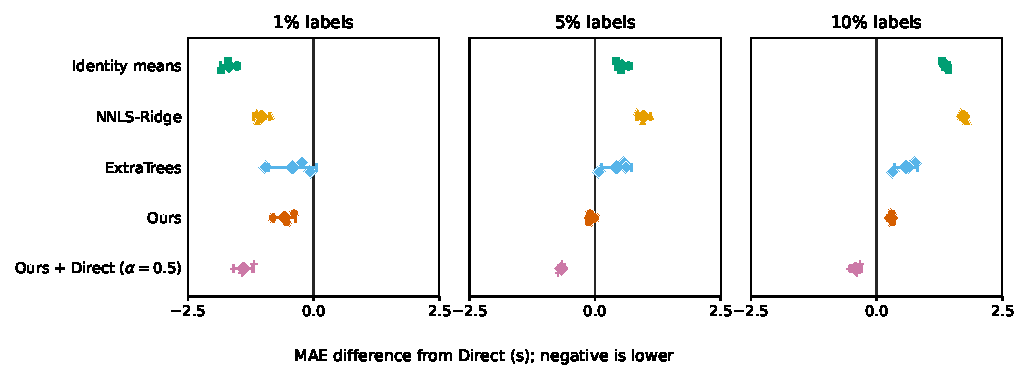
\includegraphics[width=\textwidth]{figures/followup_mae_differences.pdf}
\caption{Development-set MAE difference from direct prediction across three label layouts. Negative values indicate lower MAE. Neural results average three paired initializations within each layout; identity means and NNLS use the mean direct score for each layout, while ExtraTrees uses the paired seed-42 direct run. Points show layouts and horizontal bars show the across-layout mean and sample standard deviation.}
\label{fig:comparison}
\end{figure*}

\subsection{Label Quantity and Coverage}
Label budgets change the amount of information available for learning, but equal counts can cover different intervals. In a layout experiment with complete validation labels, restricting 23,720 training labels to the first 20\% of each trip reduces observed identities from 301 to 115 and raises our method's MAE from 28.522 to 50.121 seconds. A moving 40\% blackout retains 310 identities and gives 28.774 seconds. Prefix placement changes both positions and interval coverage, so the original comparison cannot identify position's independent effect. Full results are reported in the supplement.

\begin{table*}[t]
\centering\footnotesize\setlength{\tabcolsep}{4pt}
\caption{Label-placement control with identical identity-specific label counts; three initializations and limited validation labels. Errors in seconds. Bold marks the lowest error within each comparable group.}\label{tab:controlled_coverage}
\begin{tabular}{llrr}\toprule
Layout & Method & MAE & Prefix50\\\midrule
First 20\% & Ours & $\mathbf{50.121\pm0.938}$ & $\mathbf{318.01}$\\
First 20\% & Direct prediction & $50.472\pm0.549$ & $326.46$\\
Identity-matched random & Ours & $\mathbf{50.397\pm0.816}$ & $\mathbf{348.30}$\\
Identity-matched random & Direct prediction & $51.374\pm0.609$ & $362.85$\\
\bottomrule\end{tabular}
\end{table*}

To distinguish these changes, we use the main experiment's limited validation labels, fix the first-20\% layout, and count labels for each of its 115 intervals. A random training layout then draws \emph{exactly the same count for every interval}, totaling 23,720. Methods share validation labels, initial states, and batches. The layouts have identical interval sets and counts, while the labels occupy different trip positions.

Our method gives MAE of 50.121 seconds under prefix placement and 50.397 under matched random placement; direct prediction gives 50.472 and 51.374 (Table~\ref{tab:controlled_coverage}). Randomizing positions does not recover the roughly 29-second error with broader interval coverage, weakening an explanation that attributes all deterioration to early placement. This control uses one layout, does not fully balance trips and contexts, and selects the final update in all three matched-random fits. These results do not identify coverage's contribution independently of position.

\subsection{Correction Mechanisms and Ablations}
\begin{table*}[t]
\centering\footnotesize\setlength{\tabcolsep}{4pt}
\caption{Correction controls under a separate fixed-$\rho=0.45$, 240-update protocol across three 10\% layouts and three paired initializations per layout. Errors in seconds; mean $\pm$ sample SD. Uncentered scaling also changes effective amplitude. Bold marks the lowest error within each comparable group.}\label{tab:redistribution}
\begin{tabular}{llrrr}\toprule
Variant & $\rho$ & MAE & RMSE & Prefix50\\\midrule
Weighted centering & 0.10 & $28.849\pm0.189$ & $56.063\pm0.328$ & $145.34$\\
Weighted centering & 0.25 & $28.677\pm0.184$ & $55.503\pm0.353$ & $\mathbf{143.64}$\\
Weighted centering (fixed-$\rho$ control) & 0.45 & $28.633\pm0.239$ & $\mathbf{54.930\pm0.401}$ & $145.26$\\
Without weighted centering & 0.45 & $\mathbf{28.632\pm0.218}$ & $55.030\pm0.227$ & $143.94$\\
\bottomrule\end{tabular}
\end{table*}

We compare correction amplitudes and weighted centering under a separate fixed-$\rho=0.45$, 240-update protocol across three 10\% training/validation layouts and three paired initializations per layout (Table~\ref{tab:redistribution}). With weighted centering, $\rho=0.10$, 0.25, and 0.45 give MAE of 28.849, 28.677, and 28.633 seconds; their RMSE values are 56.063, 55.503, and 54.930 seconds. The 0.25 setting has the lowest Prefix50, so no amplitude leads on every metric. These controls are separate from the validation-selected, 960-update main comparison.

Removing weighted centering from Eq.~\eqref{eq:redistribution}, setting $r_i=b_i+\rho b_i\tanh z_i$, and applying the same total rescaling gives the following output. For $m=\sum_jp_j\tanh z_j$,
\begin{equation}
\hat t_i^{\mathrm{unc}}=T p_i\left[1+\frac{\rho(\tanh z_i-m)}{1+\rho m}\right].
\end{equation}
Compared with Eq.~\eqref{eq:shape}, rescaling also changes the effective correction amplitude. This comparison therefore tests two parameterizations without isolating centering's effect. The uncentered variant has MAE 28.632 seconds, effectively tied with the fixed-$\rho=0.45$ centered control at 28.633 seconds. Paired differences in Fig.~\ref{fig:ablation}(b)--(d) vary across metrics and runs, and these results do not establish an accuracy benefit from weighted zero-sum centering. It preserves the sum of the base estimates, while local accuracy still depends on the learned allocation.

\begin{table}[t]
\centering\footnotesize\setlength{\tabcolsep}{4pt}
\caption{Ablations with one 10\% training/validation mask and three initializations. Errors in seconds. Bold marks the lowest error within each comparable group.}\label{tab:finite_ablation}
\begin{tabular}{lrr}\toprule
Variant & MAE & Prefix50\\\midrule
Ours & $28.709\pm0.396$ & $\mathbf{144.27}$\\
No correction & $29.011\pm0.170$ & $144.66$\\
No calendar & $\mathbf{28.588\pm0.132}$ & $148.43$\\
Shuffled calendar & $29.033\pm0.153$ & $151.04$\\
\bottomrule\end{tabular}
\end{table}

Table~\ref{tab:finite_ablation} summarizes nine outcomes per condition across three 10\% training/validation layouts and three paired initializations per layout. Removing trip correction raises MAE from 28.633 to 29.038 seconds in all nine paired comparisons. Correction improves the base estimate within the same model, but this ablation does not establish an advantage of the complete method over direct prediction.

Joint calendar shuffling preserves feature combinations within each partition but breaks their association with trips; MAE rises to 29.010 seconds, with higher error than the primary model in all nine paired comparisons. Removing calendar fields gives a slightly lower mean MAE of 28.570 seconds, although RMSE and Prefix50 are higher. Mismatched information and missing information therefore have different effects, and these results do not establish that calendar features are indispensable. Both branches receive calendar context, and correction gains cannot be attributed entirely to one temporal factor.

The Singapore auxiliary experiment compares prefix-loss normalization with complete labels. Our method gives MAE of 19.518 seconds when normalization includes padding, 19.445 when it counts valid positions, and 19.490 without the prefix objective; direct prediction with valid-position normalization gives 19.545. The valid-position variant is slightly better than direct prediction and no-prefix fitting in all three pairs, but has higher long-interval error than the padding-inclusive variant. Overall and long-interval errors change differently; this complete-label experiment also differs from sparse Astana supervision.

\begin{figure}[t]
\centering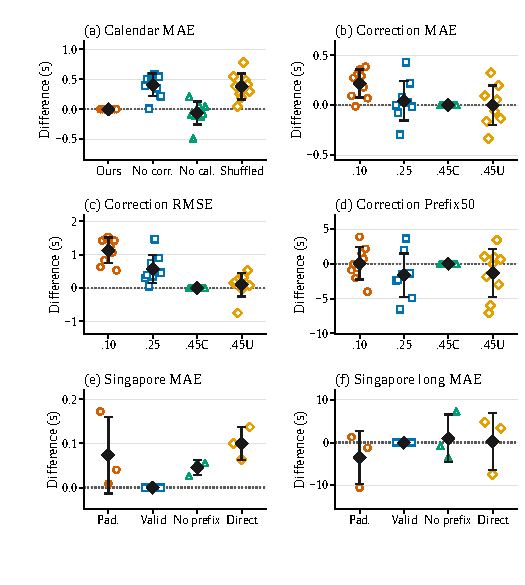
\includegraphics[width=\columnwidth]{figures/ablation_panels.pdf}
\caption{Paired error differences; positive values indicate increased error. References are Ours in (a), weighted centering with $\rho=0.45$ in (b)--(d), and valid-position prefix normalization in (e)--(f). Open markers show paired runs; filled diamonds and error bars show the mean and sample standard deviation (nine pairs per Astana condition, three per Singapore condition).}
\label{fig:ablation}
\end{figure}

\subsection{Interval Cases and Efficiency}
\begin{figure}[t]
\centering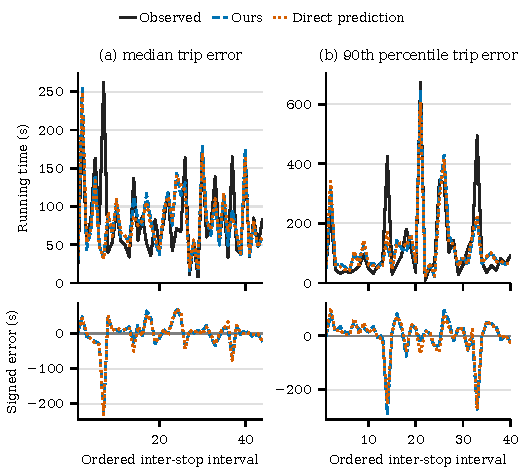
\includegraphics[width=\columnwidth]{figures/local_cases.pdf}
\caption{Development-trip interval times and signed errors. Cases nearest the median and 90th percentile of Ours trip MAE are selected from one paired run at 10\% labels. Black, blue, and orange curves show truth, Ours, and direct prediction, respectively.}\label{fig:cases}
\end{figure}
Fig.~\ref{fig:cases} shows local errors under the same total. The selected trips contain 44 and 40 intervals; their Ours/direct MAE values are 25.997/26.486 and 43.178/43.521 seconds. The larger errors are compensated by other intervals, so exact total conservation does not ensure an accurate local profile.

Timing uses the same RTX 4090 D, float32, and 256-trip batches, with ten warmups and 30 synchronized measurements. Both methods instantiate 195,079 parameters with different computation paths. The supplement reports median forward latency and interquartile ranges. Measurements include network computation and total rescaling but exclude input loading and host transfer.

\subsection{Additional Evaluation}
\begin{table*}[t]
\centering\footnotesize\setlength{\tabcolsep}{6pt}
\caption{Singapore complete-label comparison on 14,933 OD trips and 295,318 intervals. Methods without historical inputs share the supplied OD total; the strict-past reference has additional earlier-trip labels. Errors are in seconds; learned methods report mean $\pm$ population standard deviation over three runs. Bold marks the lowest error in the group without historical inputs.}
\label{tab:singapore-common-visible}
\begin{tabular}{lrrrr}
\toprule
Method & Runs & MAE (s) & RMSE (s) & Prefix50 (s)\\
\midrule
\multicolumn{5}{l}{\textit{Common-visible methods}}\\
Ours (complete labels) & 3 & $\mathbf{19.286\pm0.033}$ & $\mathbf{28.009\pm0.070}$ & $\mathbf{54.938\pm1.043}$\\
MixTTE adapter & 3 & $25.760\pm0.053$ & $35.654\pm0.171$ & $66.292\pm0.255$\\
DutyTTE adapter & 3 & $25.936\pm0.075$ & $35.823\pm0.082$ & $66.805\pm0.515$\\
TriDGNet adapter & 3 & $26.100\pm0.109$ & $36.029\pm0.117$ & $66.782\pm0.502$\\
Uniform exact projection & 1 & $34.399$ & $53.694$ & $102.362$\\
Observed-chord exact projection & 1 & $45.655$ & $60.701$ & $116.574$\\
\midrule
\multicolumn{5}{l}{\textit{History-informed reference}}\\
Strict-past direct & 1 & $19.843$ & $36.217$ & $57.385$\\
\bottomrule
\end{tabular}
\end{table*}

Table~\ref{tab:singapore-common-visible} reports a separate Singapore known-total comparison. It covers 14,933 OD trips and 295,318 segments and uses a different target definition from Astana. The common-visible methods use no same-segment history; the strict-past reference uses earlier same-segment labels and is reported separately. Ours uses the same allocation structure with complete local labels, duration weighting, and padding-inclusive prefix normalization, unlike the sparse-label Astana protocol. MixTTE, DutyTTE, and TriDGNet are task adaptations\cite{jiang2026mixtte,mao2025dutytte,zuo2026tridgnet}; their parameters and training budgets are not matched. Supplementary material gives the protocol details. These results are descriptive and are not an independent test.

After excluding dates present in training or validation, 2,060 trips and 82,783 intervals give 10\% Ours/direct MAE of 28.526/28.456 seconds. The subset of unseen complete ordered routes contains 446 trips and 17,164 intervals, with MAE of 35.963/35.315. Route-composition changes coincide with higher error, although an unseen complete route need not contain only unseen intervals.

The supplement reports seven total-bias conditions and training-budget checks. Extending the ProbETA adaptation from 960 to 3,840 updates reduces MAE from 36.403 to 32.876 seconds. One run selects the final validation point, indicating that its performance depends on the training budget.

Astana totals are derived from local labels, and labels are masked artificially. The reported scores are development results, not estimates from an untouched test set. Independent tests with measured trip totals, data from other cities, and full comparisons with native decomposition methods are needed to assess practical use and generalization.

\section{Conclusion}
We studied segment running time estimation with a known total duration, combining estimates shared across repeated intervals with current-trip adjustments. The base branch uses interval identities and context, the trip branch redistributes time within a relative bound, and final rescaling enforces the supplied total. Outputs remain nonnegative and sum-consistent, although the total constraint alone cannot guarantee interval accuracy.

Segment means remain competitive with very few labels. Ours has lower point-estimate MAE than direct prediction at 1\% and 5\% (by 0.579 and 0.075 seconds), but higher MAE at 10\%; paired runs favor Ours in eight, six, and zero of nine cases. Its long-interval MAE is higher at every budget. The validation-selected Ours+Direct ensemble has the lowest mean MAE at 5\% and 10\%, while segment means remain better at 1\%, but the ensemble is a separate predictor. These development results do not establish a uniform advantage for Ours. Equal label counts also yield different errors under different interval coverage. Independent totals, an unopened external evaluation, and data from other cities are needed to determine whether the allocation structure improves local estimates beyond these development comparisons.

\bibliographystyle{IEEEtran}
\bibliography{references,additional_references}
\end{document}
